\documentclass[11pt]{article}
\usepackage[a4paper,margin=1in]{geometry}
\usepackage[T1]{fontenc}
\usepackage{lmodern}
\usepackage{microtype}
\usepackage{booktabs}
\usepackage{graphicx}
\usepackage{amsmath}
\usepackage[numbers,sort&compress]{natbib}
\usepackage{xcolor}
\usepackage[colorlinks=true,linkcolor=black,citecolor=teal!70!black,urlcolor=teal!70!black]{hyperref}
\usepackage{caption}
\captionsetup{font=small,labelfont=bf}
\hypersetup{pdftitle={What a Local Screen Could Not Tell Us: Measuring a Small Offline Coding Agent Under a Twelve-Hour Budget},pdfauthor={Carson Rodrigues}}

\title{What a Local Screen Could Not Tell Us:\\Measuring a Small Offline Coding Agent Under a Twelve-Hour Budget}
\author{Carson Rodrigues\\[2pt]
\small Celabe Research \quad \texttt{carson@celabe.com} \quad ORCID \href{https://orcid.org/0009-0001-7195-6742}{0009-0001-7195-6742}}
\date{October 2026}

\begin{document}
\maketitle

\begin{abstract}
In the Gemma 4 Developer Agent competition the model, the tools and the scorer are fixed, and an entry is only an agent
configuration: its prompt, its limits and its sampling settings. Entrants choose between configurations the way most agent
builders do, by running them on a small public task set before spending a scarce hidden submission. We report what that
practice told us over four weeks, from 20 complete runs on the 74 public tasks across two local setups (the scorer's own
four-L4 hardware and a single GPU paced to it) and 11 configurations submitted to the hidden set. The local screen was a poor guide.
On the scorer's hardware, a change that beat its parent on nine tasks and lost none scored lower on the hidden set. On the
paced GPU, three configurations that each solved 28 of 74 locally scored 0.10, 0.10 and 0.17, and the rank correlation
between local and hidden scores was $+0.49$ (exact permutation $p=0.32$, seven configurations). Three measurements explain
much of this. Between 91 and 97 percent of each task's wall time is the model generating text, so the per-task time cap is a
token budget. Solves arrive late, so longer caps buy local solves that a hard twelve-hour limit on the whole run cannot pay
for: a public configuration that scored 0.24 for its author ran out of time on both of our attempts. And prompt rules that each
fixed one task lost seven tasks when merged. We also ran Google's Harness$^2$ with Gemma as its own harness improver: 23 of 30
improver sessions overflowed the model's 32k context and no change to the harness was adopted. Every reading rule was committed to
git before its result, every number is regenerated from saved files, and all code and data are public.
\end{abstract}

\section{Introduction}

Agent benchmarks are usually reported as a single pass rate on a public set. Builders, though, use benchmarks differently: as
a filter that decides which of several close variants to ship. The question that matters to them is not whether a set is
hard, but whether a gain on it predicts a gain where it counts. That question is rarely measured, because the place where it
counts is usually not available to measure.

The Gemma 4 Developer Agent competition on Kaggle \citep{kaggle2026gemma4} makes it measurable. The model, its quantisation,
the serving stack, the tool set and the scorer are fixed by the organisers. An entrant submits an agent configuration, and
the scorer runs it once on each of about 120 hidden tasks drawn from private repositories, in sequence, on four L4 GPUs, under
a twelve-hour limit for the whole run. About 58 of those tasks form a public leaderboard, so one task moves the public score
by about 0.017, and one submission is allowed per day. Every entrant therefore faces the same daily decision with the same
tools: which configuration, among those that look good on the 74 public tasks, should spend the next hidden read?

This paper is a measurement of that decision, taken from our own entry. Its contributions are:

\begin{itemize}
\item \textbf{A calibration of local screens against a hidden set} (Section~\ref{sec:calibration}). Two local screens, one on
the scorer's hardware and one on a paced GPU, compared against the hidden results of 11 configurations. Neither ranked them usefully,
and the most convincing local wins did not transfer.
\item \textbf{Three mechanisms behind the mismatch} (Sections~\ref{sec:budget}--\ref{sec:merge}): the time cap is a token
budget; solves arrive late, which couples the per-task cap to a per-run time limit; and rules that fix single tasks cost more
on the population than they fix.
\item \textbf{A reading protocol that can be checked from the outside} (Section~\ref{sec:method}): every rule for reading a
run was committed before the run, and a script proves the order from git history.
\item \textbf{A negative result on automatic harness improvement with a small model} (Section~\ref{sec:harness2}): with
Gemma as its own improver in a 32k context, Harness$^2$ \citep{xu2026harness2} adopted no change to the harness, and an audit of
its sessions shows why.
\end{itemize}

The numbers are small, and we say so throughout. The point is not that local screens are useless in general. It is that in
one well-controlled setting, with the model fixed and the hardware matched, a screen of this size did not carry the
information builders routinely assume it does, and the reasons are mechanical rather than mysterious.

\section{Setting}
\label{sec:setting}

\paragraph{Fixed parts.} The model is Gemma 4 31B, instruction tuned and quantised to 4-bit weights with 16-bit activations,
served by vLLM with a 32{,}768-token context. The agent framework is Google's ADK; the scorer compacts the conversation when it
passes about 14k tokens. The tools are fixed: run a shell command (300 s and 5{,}000 characters of output at most), read,
edit and write files, query a code graph, and submit a patch. A task is a real issue in a real Python repository; it counts
as solved when every hidden test of that issue passes after the agent's patch is applied, with any test files the agent
touched reset first.

\paragraph{What an entrant controls.} The system prompt, optional skills (scripts and documents the agent can call), the
per-task limits (wall-clock minutes, tool calls, turns, per-command timeout), the sampling settings (temperature, top-$p$,
thinking budget) and, in principle, a LoRA adapter. Nothing else. Every idea has to be paid for in the model's own time.

\paragraph{The two sets.} The 74 public tasks come from four repositories (fastapi, rich, requests, httpx). The hidden
tasks come from private repositories. The scorer runs the hidden tasks one at a time; if the whole run exceeds twelve hours,
the submission scores nothing.

\section{Method}
\label{sec:method}

\subsection{Two local screens}
We ran configurations locally in two ways. Early on, on Kaggle's own four-L4 notebooks, the scorer's hardware. Later, when
we needed more runs than that quota allowed, on a single A6000 at a university lab, with the same weights and serving stack.
On the A6000 a small proxy holds every model reply until the time it would have taken on four L4s has passed. Its timing
model was fitted to 6{,}730 model calls timed on Kaggle's L4s (decode at 33--36 tokens per second for one stream, prefill
at about 1{,}400--1{,}700 tokens per second). A five-minute cap therefore buys the same amount of model work on both setups.
During a task the paced A6000 produced about 29 generated tokens per second of wall time.

Every local screen ran all 74 public tasks, once each, in a fixed order. We never judged a change on a subset.

\subsection{Configurations}
Appendix Table~\ref{tab:runs} lists every complete local run. The configurations that matter here are few. The
\emph{baseline} (\texttt{v12}) is one agent with thinking on, a 5-minute cap, 40 tool calls and a short procedural prompt.
\emph{Public sampling} (\texttt{v12b}) is the baseline with the sampling block of the best public notebook (temperature 0.2,
top-$p$ 0.95, no top-$k$, no seed). The \emph{public 0.24 notebook} (\texttt{pub024}) is that notebook, byte for byte, kept as
a control: its author's single draw scored 0.24, at the time the top of the leaderboard. Two prompt rules, L1 (edit only
through a shell heredoc, with the edit tools removed) and L2 (a 60-second per-command timeout), appear in several variants.

\subsection{Reading rules, committed first}
Before each run we wrote down, in an append-only log kept in git, what result would make us ship, drop or retest the
configuration, and how its hidden score would be read. A script resolves each rule to the commit that first added it and each
result to the commit (or Kaggle submission time) that first recorded it, and checks that the rule came first. Results that no
rule anticipated are labelled \emph{post hoc} below. Two kinds of correction are recorded rather than hidden: one in-place edit
of three heading timestamps (disclosed in the log) and a later rewrite of commit author emails before the repository went
public, which changed every commit hash but kept dates and contents; a published map translates old hashes to new.

\subsection{Comparisons}
Two configurations are compared task by task: how many tasks only A solved, how many only B solved, and an exact two-sided
sign test on those two counts. Totals alone hide how much moved. Hidden scores are single numbers per submission, so they
are compared against the spread of repeated submissions of one configuration (Section~\ref{sec:repeats}).

\section{Results}

\subsection{How much a repeat moves}
\label{sec:repeats}

Two configurations were run twice each on the paced A6000, unchanged (Table~\ref{tab:repeats}). Their totals moved by two
tasks each time, but four and six tasks flipped, in both directions. Only 13 and 4 of the 74 runs replayed step for step;
the agent usually reached the same outcome by a different path, even with a fixed sampling seed. We had written down before
the second repeat that more than eight flips would widen the noise floor we used for every later comparison; it stayed at six.

Four configurations went to the hidden set twice (post hoc for the first three, pre-registered for the last). They came back
zero to one task apart. That agrees with the local repeats: when a few tasks flip each way, two totals land close together.
A small gap between two totals does not mean few tasks changed, and a single hidden score cannot show which ones did.

\begin{table}[t]
\centering\small
% generated by paper/arxiv/make_tex_tables.py
\begin{tabular}{lrrrr}
\toprule
configuration & solves & flips (gained/lost) & sign $p$ & exact replays \\
\midrule
v13 & 31, 29 & 4 (1/3) & 0.625 & 13 \\
v12 (baseline) & 27, 29 & 6 (4/2) & 0.688 & 4 \\
\bottomrule
\end{tabular}

\vspace{6pt}

% generated by paper/arxiv/make_tex_tables.py
\begin{tabular}{lr}
\toprule
configuration & hidden public reads \\
\midrule
v4 (old scorer) & 0.12, 0.12 \\
v10.1 & 0.08, 0.08 \\
v4h2 (edit helper) & 0.10, 0.08 \\
v12 (baseline) & 0.15, 0.13 \\
\bottomrule
\end{tabular}

\caption{Repeats. Top: the same configuration run twice on the paced A6000 (74 tasks). Bottom: the same configuration
submitted twice to the hidden set. The first pair predates a rebuild of the scorer; each pair is within one scorer version.}
\label{tab:repeats}
\end{table}

\subsection{Neither local screen ordered the hidden scores}
\label{sec:calibration}

\begin{figure}[t]
\centering
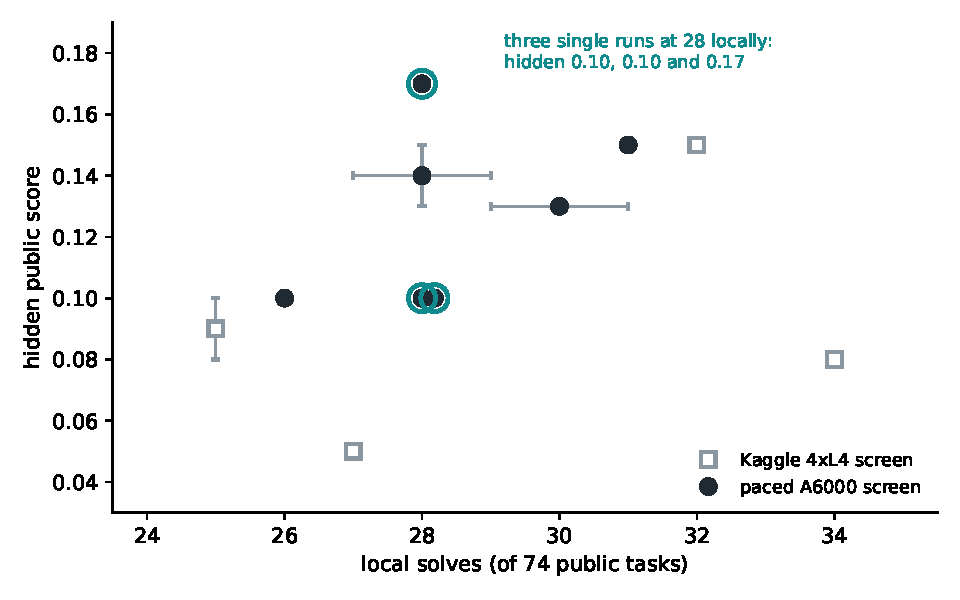
\includegraphics[width=0.78\linewidth]{figures/calibration.pdf}
\caption{Local solves against hidden public score. Bars span repeated runs or repeated hidden reads of one configuration.
Hollow squares are runs on Kaggle's own 4xL4 hardware; filled circles are runs on the paced A6000. Not shown: the public
0.24 notebook, which solved 31 locally and exceeded the twelve-hour limit on both hidden attempts.}
\label{fig:calibration}
\end{figure}

Figure~\ref{fig:calibration} and Table~\ref{tab:calibration} put every configuration with both a full local run and a
hidden score side by side.

On the scorer's own hardware, four configurations had both. One of them, a recovery step for failed helper calls, looked like
a clean win: against its parent it solved nine more tasks and lost none ($p=0.004$). We had written down before submitting it
that five to seven hidden tasks would read as noise. It scored 0.08, five tasks, against its parent's 0.10 and 0.08. The
local best was the hidden third, and the rank correlation over the four configurations was 0.00.

On the paced A6000, seven configurations had hidden scores. The rank correlation between local and hidden scores was $+0.49$,
with an exact permutation $p$ of $0.32$ over seven configurations: positive, but indistinguishable from no relation at this
size. The decisions it would have made were wrong in a specific way. Three configurations solved exactly 28 locally and
scored 0.10, 0.10 and 0.17 on the hidden set, the lowest and the highest hidden scores among the paced-GPU configurations. The two local leaders, at 31,
scored 0.13 and 0.15, and the public notebook, also at 31, scored nothing. (The A6000 comparison was assembled after the
fact; the L4 reading was written down first.)

This does not show that the hidden score is right and the local screen wrong: a 0.05 gap is three hidden tasks, and most
configurations have one hidden draw. It shows something narrower and more useful. Inside the band where all our
configurations lived, a 74-task screen did not separate them, on the scorer's own hardware or on a matched one.

\begin{table}[t]
\centering\small
% generated by paper/arxiv/make_tex_tables.py
\begin{tabular}{lrr}
\toprule
configuration & local solves (of 74) & hidden public \\
\midrule
staged agent & 27 & 0.05 \\
+ edit helper & 25 & 0.10, 0.08 \\
+ recovery step & 34 & 0.08 \\
baseline (on L4) & 32 & 0.15 \\
\bottomrule
\end{tabular}

\vspace{6pt}

% generated by paper/arxiv/make_tex_tables.py
\begin{tabular}{lrr}
\toprule
configuration & local solves (of 74) & hidden public \\
\midrule
thinking-only variant & 26 & 0.10 \\
thinking budget 1,024 & 28 & 0.10 \\
public sampling + heredoc edits, 60 s commands & 28 & 0.10 \\
baseline & 27, 29 & 0.15, 0.13 \\
baseline + public sampling & 28 & 0.17 \\
baseline + two prompt rules & 31, 29 & 0.13 \\
public sampling + 6-minute cap & 31 & 0.15 \\
public 0.24 notebook (8-min cap) & 31 & 12-h limit exceeded, 2 of 2 \\
\bottomrule
\end{tabular}

\caption{Local solves and hidden public scores. Top: Kaggle's 4xL4 notebooks (scorer hardware). Bottom: the paced A6000,
sorted by local solves. Configurations with two numbers were run or submitted twice.}
\label{tab:calibration}
\end{table}

\subsection{The time cap is a token budget}
\label{sec:budget}

We split each task's wall time into model calls and everything else, from the traces of ten A6000 runs
(Figure~\ref{fig:timesplit}, post hoc). Model generation took 91 to 97 percent; earlier traces from Kaggle's L4s gave 91
to 93. A typical task made about 22 model calls and generated about 7{,}500 tokens. At the 29 tokens per second we see during
a task, a five-minute cap is a budget of roughly 8{,}700 generated tokens. Anything that makes the model write more spends it:
longer thinking, a longer prompt to re-read, a wordier edit format. Faster tools would save almost nothing.

\begin{figure}[t]
\centering
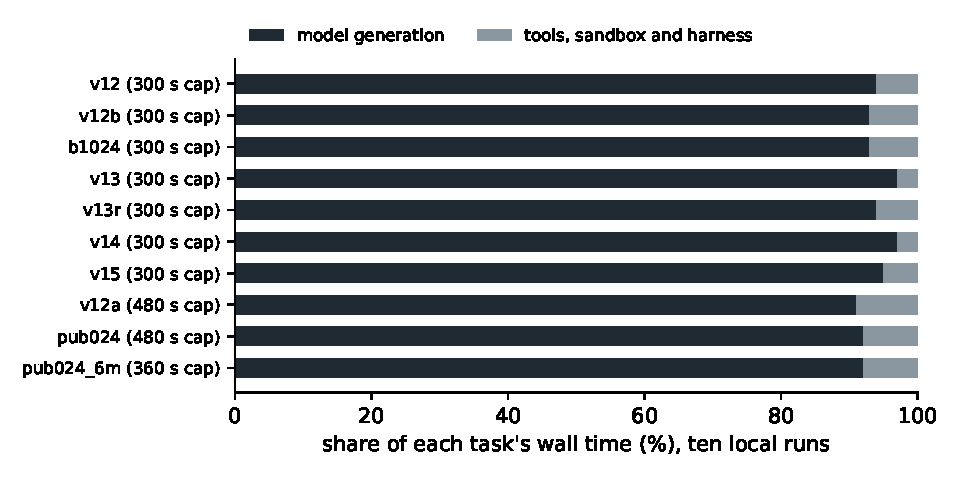
\includegraphics[width=0.78\linewidth]{figures/timesplit.pdf}
\caption{Where each task's time goes, in ten local runs: model generation against everything else (tool execution, sandbox,
harness). Identifiers are listed in Appendix Table~\ref{tab:runs}.}
\label{fig:timesplit}
\end{figure}

\subsection{Solves arrive late}
\label{sec:late}

In the baseline, 41 of 74 tasks ran until the five-minute cap. Seven of its 27 solves ended in the last 30 seconds, and four
were still running when the cap hit; the scorer grades whatever edit exists at that moment. Figure~\ref{fig:deadline} shows
how many solves each configuration would keep under a shorter cap, counting a solve only if its run ended before the cutoff
(post hoc).

The public 0.24 prompt makes this much stronger. Given eight minutes, it solved 31 tasks locally, but only 19 of those ended
before the five-minute mark. The same prompt on our tools behaved the same way: 32 solves at eight minutes, 16 by five. A
thorough prompt pays for its solves in minutes.

The extra minute is a real lever locally. Our baseline with public sampling and a six-minute cap solved 31 of 74, three more
than the same configuration at five minutes, and four of the five tasks it gained ended after the five-minute mark. On the hidden
set it scored 0.15, one task below the five-minute version's 0.17.

\begin{figure}[t]
\centering
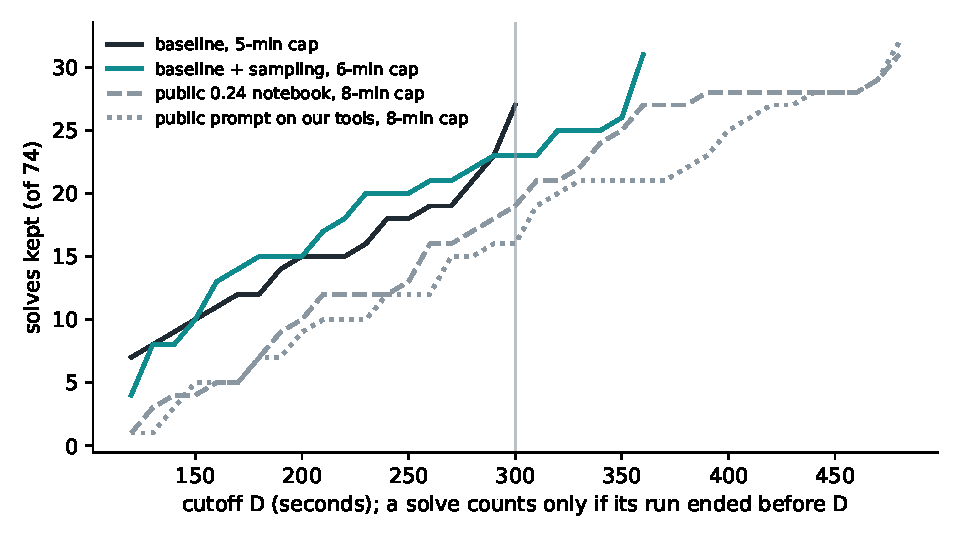
\includegraphics[width=0.78\linewidth]{figures/deadline.pdf}
\caption{Solves kept if the per-task cap were the cutoff on the horizontal axis (conservative: a solve counts only if its
run ended at least 5 s before the cutoff, except at the configuration's own cap). The vertical line marks five minutes.}
\label{fig:deadline}
\end{figure}

\subsection{The twelve-hour limit is per run}
\label{sec:runtime}

The public notebook averaged 346 seconds per task on the paced A6000. Over 120 tasks that is 11.5 hours, inside the limit on
paper. Both of our hidden attempts ran out of time and scored nothing; its author's attempt scored 0.24. The same
configuration can pass or fail. Our rule for that submission had not anticipated a failure at all, so this outcome is reported
as unforeseen.

The mechanism follows from Sections~\ref{sec:budget} and~\ref{sec:late}. A configuration whose solves come late spends most
of its cap on many tasks, and a hidden set with slower or harder tasks than the public one pushes the total past twelve hours.
We replaced our mean-time gate with a worst-case one (120 tasks times the per-task cap must fit in ten hours), which only
five-minute configurations pass. Later, by a deliberate amendment, we sent one six-minute configuration with a measured mean of
280.3 seconds per task; it finished inside the limit. Every configuration in Table~\ref{tab:calibration} with a five- or six-minute cap
scored; both eight-minute attempts did not.

\subsection{Fixes that worked one task at a time lost when merged}
\label{sec:merge}

We tried a per-task approach: find a task the agent fails, write one prompt rule aimed at that failure, and keep the rule
only if it solves its target in at least two of three tries. Two rules passed: one solved its target three times out of
three, the other two out of two. Merged into one configuration, they lost seven tasks net on the full 74 (gained one, lost
eight; $p=0.04$). Each rule fixed its own task; together they cost more elsewhere than they fixed, and only the full 74 showed
it.

\subsection{Moving toward the public best, one change at a time}
\label{sec:steps}

Our baseline and the public 0.24 notebook differ in three ways: limits, sampling and prompt. We moved the baseline toward it
one difference at a time, each a full local run paired against the baseline (Table~\ref{tab:steps}). Our rule called a change
real at a net of three tasks or more. By that rule only the prompt passed, and only together with the eight minutes it was
written for: restated for five minutes, the same prompt lost ten tasks against its eight-minute version ($p=0.006$). The
public prompt needs its eight minutes, and eight minutes fails the twelve-hour gate.

The hidden set then gave a different ranking of the same levers. The sampling change, neutral locally ($+1$), produced our best
hidden score (0.17 against the baseline's 0.15 and 0.13). Adding L1 and L2 to it, neutral locally (28 against 28, three tasks
gained and three lost), dropped the hidden score to 0.10.

\begin{table}[t]
\centering\small
% generated by paper/arxiv/make_tex_tables.py
\begin{tabular}{lrrrrrr}
\toprule
change & A & B & only A & only B & net & sign $p$ \\
\midrule
public limits (8 min, 28 calls) & 29 & 27 & 8 & 6 & $+2$ & 0.791 \\
public sampling (temperature 0.2) & 28 & 27 & 3 & 2 & $+1$ & 1.000 \\
public limits and prompt & 32 & 27 & 7 & 2 & $+5$ & 0.180 \\
public prompt restated for 5 min & 22 & 27 & 2 & 7 & $-5$ & 0.180 \\
\quad same prompt: 5 min vs 8 min & 22 & 32 & 1 & 11 & $-10$ & 0.006 \\
public notebook cut to 6 min & 25 & 31 & 1 & 7 & $-6$ & 0.070 \\
\bottomrule
\end{tabular}

\caption{Moving the baseline toward the public 0.24 notebook one difference at a time (74 tasks each). A and B are the two
runs compared; ``only A'' counts tasks A solved and B did not.}
\label{tab:steps}
\end{table}

\subsection{A shared GPU can fake a result}
\label{sec:contention}

One local run was invalid for a reason unrelated to the agent (post hoc). During a daytime run on the shared A6000, another
process on the host took GPU memory, the driver most likely began paging, and the model server stalled for minutes at a time.
Eleven of 56 rows recorded zero model calls; to the scoring script they looked like an agent that gave up. We stopped the
run, marked it contaminated, lowered the server's memory share, and added a rule: a row with no model calls while the server
answered nothing is an infrastructure loss, rerun separately, never a result.

\section{Letting a model improve the harness}
\label{sec:harness2}

Harness$^2$ \citep{xu2026harness2} refines an agent's harness task by task. An improver model reads the agent's trajectories,
proposes edits from two angles (task-invariant and domain-specific), tests them in fresh runs, composes a final harness, and
stores a lesson for the next task. By default the same model acts as executor and editor. We wrote an
adapter that maps the competition's agent format onto Harness$^2$'s editable surface and runs every rollout through the same
paced sandbox as our local screens. We ran it with Gemma as the fixed solver on eight held-out tasks from one repository
(arrow), with Gemma itself as the improver first, the framework's default. The task list, the reading rules and the spending
caps were committed before the first rollout.

Gemma did not change the harness. By the pre-registered rules the mechanics passed (every stage returned a valid harness and
no rollout crashed on all eight tasks), no harness was adopted, and there was no signal: the chosen runs solved two tasks
against one for the unchanged harness, and both solutions came from the unchanged harness itself. The improver kept the
original in 22 of 24 stages.

Reading its sessions shows why (Table~\ref{tab:h2}, post hoc). Twenty-three of the 30 improver sessions ran past Gemma's 32k
context and were cut down by the coding agent that hosts them, after which they summarised the task and stopped; one ended by
asking whether it should begin. Of the seven that fit, four replied with the bare words ``keep base'', one edited the
repository instead of the harness, and two produced the only changed harnesses. ``Kept the base'' therefore mostly records a
session that never acted, not a judgement that the base was good. The pre-registration had named this failure mode in advance
as a possible Phase~1 result.

Two further phases were pre-registered and did not run: the same eight tasks with three frontier improvers that have no 32k
limit, and a transfer test of anything they adopted on 12 tasks from two repositories they never saw. The lab GPU was
returned before the API key for the frontier improvers was in place. We report that plainly rather than leave the design
implying results.

\begin{table}[t]
\centering\small
% generated by paper/arxiv/make_tex_tables.py
\begin{tabular}{lrrr}
\toprule
stage & sessions & overflowed 32k & bare ``keep base'' \\
\midrule
propose (invariant) & 8 & 4 & 3 \\
propose (domain) & 8 & 5 & 1 \\
compose & 8 & 8 & 0 \\
reflect & 6 & 6 & 0 \\
\midrule
all & 30 & 23 & 4 \\
\bottomrule
\end{tabular}

\caption{Harness$^2$ improver sessions with Gemma 4 31B as its own improver (eight tasks). ``Overflowed'' counts sessions
whose reply shows the host agent's context-compaction notice.}
\label{tab:h2}
\end{table}

\section{What this changes in practice}
\label{sec:practice}

We changed how we used the local screen, and the change generalises beyond this competition.

\paragraph{Use a local screen as a gate, not a ranker.} It still does two jobs well: catching broken configurations
(crashes, errors, malformed edits, leaks into the patch, how many tasks hit the cap) and setting a floor. Within the band where
working configurations live, it should not choose between them unless its size has been checked against repeats.

\paragraph{Spend hidden reads on mechanisms, one at a time.} Each scarce hidden read should carry a single change with a
stated mechanism and a reading rule written beforehand, never a change chosen because it won a local screen by two tasks.

\paragraph{Repeat on purpose, locally and remotely.} Two runs of one configuration measure how far apart two numbers must be
before they mean anything. Our repeats moved totals by two tasks while flipping four to six; that is the scale below which
local differences are noise.

\paragraph{Budget in tokens and in worst cases.} When generation dominates wall time, the per-task cap is a token budget,
and a per-run time limit makes the worst case, not the mean, the binding constraint.

\section{Threats to validity}
\label{sec:threats}

Everything here concerns one fixed model, one agent framework, one competition's scorer and 74 public tasks from four
repositories. The hidden columns have one or two draws per configuration on about 58 tasks, so single hidden differences of one
task are within the spread we measured. The rank correlations are computed over seven and four configurations and have wide
uncertainty. The pacing proxy models the scorer's speed rather than being the scorer, which is why the L4 results matter. The
scorer was rebuilt by the organisers in late September; we compare hidden scores only within one scorer version. Several
results were noticed after the runs (marked post hoc); the rest were read against rules committed before the run. The
competition's configurations differ from each other in small ways, and a screen might rank larger differences correctly;
we tested the regime builders actually work in.

\section{Related work}
\label{sec:related}

Our setting follows SWE-bench \citep{jimenez2024swebench}: an issue and a repository in, a patch out, judged by the
repository's tests. SWE-agent \citep{yang2024sweagent} showed that the interface between model and repository changes an
agent's score, the premise of this competition. Agentless \citep{xia2025agentless} showed that a fixed, cheap pipeline can
compete with free-form agents, and SWE-Effi \citep{fan2025sweeffi} scores agents against token and time budgets; our
Section~\ref{sec:budget} is a budget result of the same kind.

Run-to-run noise in agent evaluation is measured by \citet{bjarnason2026randomness}, who ran 60{,}000 SWE-bench Verified
trajectories and found single-run pass@1 moving by 2.2 to 6.0 points depending on the run picked, with spread even at
temperature zero; they recommend several runs per task and a power analysis. \citet{kapoor2024agents} argue for reporting cost
with accuracy and for holdouts that agents cannot overfit, and \citet{zhu2025abc} show that benchmark flaws can badly misstate
agent performance. On leaderboards, \citet{blum2015ladder} show how repeated public queries overfit a holdout, while
\citet{roelofs2019meta} found little such overfitting across more than 100 Kaggle competitions. Our disagreement between a
local screen and a hidden set is a different problem, closer to the private-repository split of SWE-Bench Pro
\citep{deng2025swebenchpro} and to fresh-task benchmarks such as SWE-bench-Live \citep{zhang2025swebenchlive} and
SWE-rebench \citep{badertdinov2025swerebench}.

For automatic harness improvement: Harness$^2$ \citep{xu2026harness2}, Meta-Harness \citep{lee2026metaharness},
Self-Harness \citep{zhang2026selfharness}, MESH-Harness \citep{shang2026mesh}, Agentic Harness Engineering
\citep{lin2026ahe}, HarnessOpt-Bench \citep{ursekar2026harnessopt} and the adaptation of harnesses for small models by
\citet{yang2026better}. \citet{wang2026rethinking} find that harness evolution does not beat simple test-time scaling at
matched budgets and warn against evolving on the benchmark's own tests; our adapter keeps the improver away from the tests,
which are used only to grade after selection.

\section{Conclusion}

With the model, tools, scorer and hardware held fixed, a 74-task local screen did not tell us which of our agent
configurations would score best on a hidden set from other repositories. The reasons were mechanical: noise of a few tasks
per run, a time cap that is really a token budget, solves that arrive late and collide with a per-run time limit, and fixes
that help one task while costing the population. A small model asked to improve its own harness, in its own context window,
did not act at all. The practical lesson is modest and, we think, general: measure the spread of your screen before you let
it choose for you, and spend scarce evaluations on one stated mechanism at a time.

\section*{Reproducibility}
\begin{sloppypar}
All configurations, per-task results, traces, the append-only reading-rule log, the analysis scripts and the source of this
paper are at \url{https://github.com/rodriguescarson/gemma-swe-agent} (Apache-2.0). \texttt{python3 paper/arxiv/make\_figures.py}
and \texttt{python3 paper/arxiv/make\_tex\_tables.py} regenerate every figure and table here from the saved results;
\texttt{eval/analysis/check\_claims.py} checks that each reading rule was committed before its result.
\end{sloppypar}

\section*{Acknowledgements and disclosure}
The local screens ran on a lab A6000 made available through the author's university network. The engineering, the analysis
scripts and the drafting of this paper were carried out with an AI coding assistant (Claude Code); every number in the paper
is regenerated from saved results by the scripts above and was checked by the author, who takes responsibility for the work.

\bibliographystyle{plainnat}
\bibliography{refs}

\appendix
\section{Every complete local run}
\begin{table}[h]
\centering\footnotesize
% generated by paper/arxiv/make_tex_tables.py
\begin{tabular}{llrrrr}
\toprule
id & configuration & cap (s) & solved & mean s & 120-task h \\
\midrule
\texttt{v0-think} & starter agent with thinking on & 300 & 26 & 265 & 8.8 \\
\texttt{v12} & baseline: one agent, thinking on & 300 & 27 & 251 & 8.4 \\
\texttt{v12} & baseline, second run & 300 & 29 & 260 & 8.7 \\
\texttt{v12-b1024} & baseline, thinking budget 1,024 & 300 & 28 & 251 & 8.4 \\
\texttt{v13} & b1024 + two prompt rules (L1, L2) & 300 & 31 & 253 & 8.4 \\
\texttt{v13} & same, second run & 300 & 29 & 252 & 8.4 \\
\texttt{v14} & v13 + two per-task rules & 300 & 24 & 261 & 8.7 \\
\texttt{v15} & baseline + L1 + L2 & 300 & 29 & 259 & 8.6 \\
\texttt{v12a} & baseline + public limits (8 min) & 480 & 29 & 314 & 10.5 \\
\texttt{v12b} & baseline + public sampling & 300 & 28 & 247 & 8.2 \\
\texttt{v12c} & baseline + public limits and prompt & 480 & 32 & 354 & 11.8 \\
\texttt{v16} & baseline + public prompt at 5 min & 300 & 22 & 281 & 9.4 \\
\texttt{pub024} & public 0.24 notebook, unchanged & 480 & 31 & 346 & 11.5 \\
\texttt{pub024-6m} & public notebook at 6 min & 360 & 25 & 313 & 10.4 \\
\texttt{v12b6} & v12b with a 6-minute cap & 360 & 31 & 280 & 9.3 \\
\texttt{v15b} & v12b + L1 + L2 & 300 & 28 & 250 & 8.3 \\
\bottomrule
\end{tabular}

\caption{All complete 74-task runs on the paced A6000. ``120-task h'' projects the mean seconds per task onto a 120-task
hidden run.}
\label{tab:runs}
\end{table}

\end{document}
